\section{Spinpräzession im Erdmagnetfeld}
\subsection{Durchführung}
Die Bestimmung der Spinpräzession im vertikalen Erdmagnetfeld erfolgt folgendermaßen:
Das \textlambda/4-Plättchen im Strahlengang erzeugt zirkular polarisiertes Licht,
durch das die Rubidiumatome im Magnetfeld optisch gepumpt werden.
Das Magnetfeld wird von Spule~5 erzeugt, ihre Stromversorgung erfolgt vom \emph{instec function~generator}.
Der Funktionsgenerator erzeugt ein Rechtecksignal mit einer Spitze-zu-Spitze-Amplitude von 26\,mV und
einem Offset von 13\,mV, sodass das Magnetfeld periodisch an- und ausgeschaltet wird.
Um das Erdmagnetfeld in Strahlrichtung zu kompensieren,
wird ein Strom von $I_1$=17\,mA durch Spule~1 geschickt.
Die Temperatur des Peltierelements beträgt bei den Messungen 33.9$^\circ$C.
Es werden zuerst zwei Messreihen durchgeführt, um die beiden Rubidiumisotope zu untersuchen:
Mit 63.7\,mA Laserstrom (Pumpen von \rb{85}) und mit 64.1\,mA (\rb{87}).
Während einer Messreihe wird der Strom durch Spule~4 zwischen 0\,mA und 100\,mA variiert und
so die Vertikalkomponente des Magnetfelds beeinflusst
(eine Kompensation des vertikalen Erdmagnetfeldes findet bei ca. 90\,mA statt).
Das Transmissionssignal der Messzelle wird mit dem Oszilloskop gemessen und
es findet eine Heizung mit dem Föhn statt.

Nach Durchführung der ersten beiden Messungen wurde festgestellt,
dass mit der Variation des Stroms durch Spule~4 keine vollständige Kompensation des Magnetfelds möglich ist.
(Eine vollständige Kompensation würde sich darin zeigen,
dass die Frequenz der Spinpräzession sehr groß wird und keine Präzession mehr messbar ist).
Dies wurde auf die Anwesenheit der Horizontalkomponente des Erdmagnetfeldes
senkrecht zum Strahlengang zurückgeführt, da der Messaufbau nicht parallel zum Horizontalanteil des
Erdmagnetfelds ausgerichtet ist und durch Spule~1 nur ein Magnetfeld parallel zum Strahlengang kompensiert wird.

Aus dem Anteil des Magnetfelds, das bei den ersten beiden Messreihen nicht kompensierbar war
(dieser Anteil wurde mit einem Modell bestimmt, das an die Messdaten angepasst wurde),
konnte die Winkelabweichung des Messaufbaus von der Nordausrichtung vorhergesagt werden.
Der Messaufbau wurde um den so bestimmten Winkel gedreht und eine weitere Messreihe an \rb{85} durchgeführt,
um eine vollständige Magnetfeldkompensation und ein Verschwinden der Spinpräzession zu erreichen.
Zusätzlich wurde bei einem Strom von 90\,mA durch Spule~4 die Winkelabhängigkeit der Präzessionsfrequenz untersucht,
indem diese für verschiedene Ausrichtungen des Strahlengangs gemessen wurde.

\subsection{Auswertung}

\begin{figure}[H]
    \begin{center}
        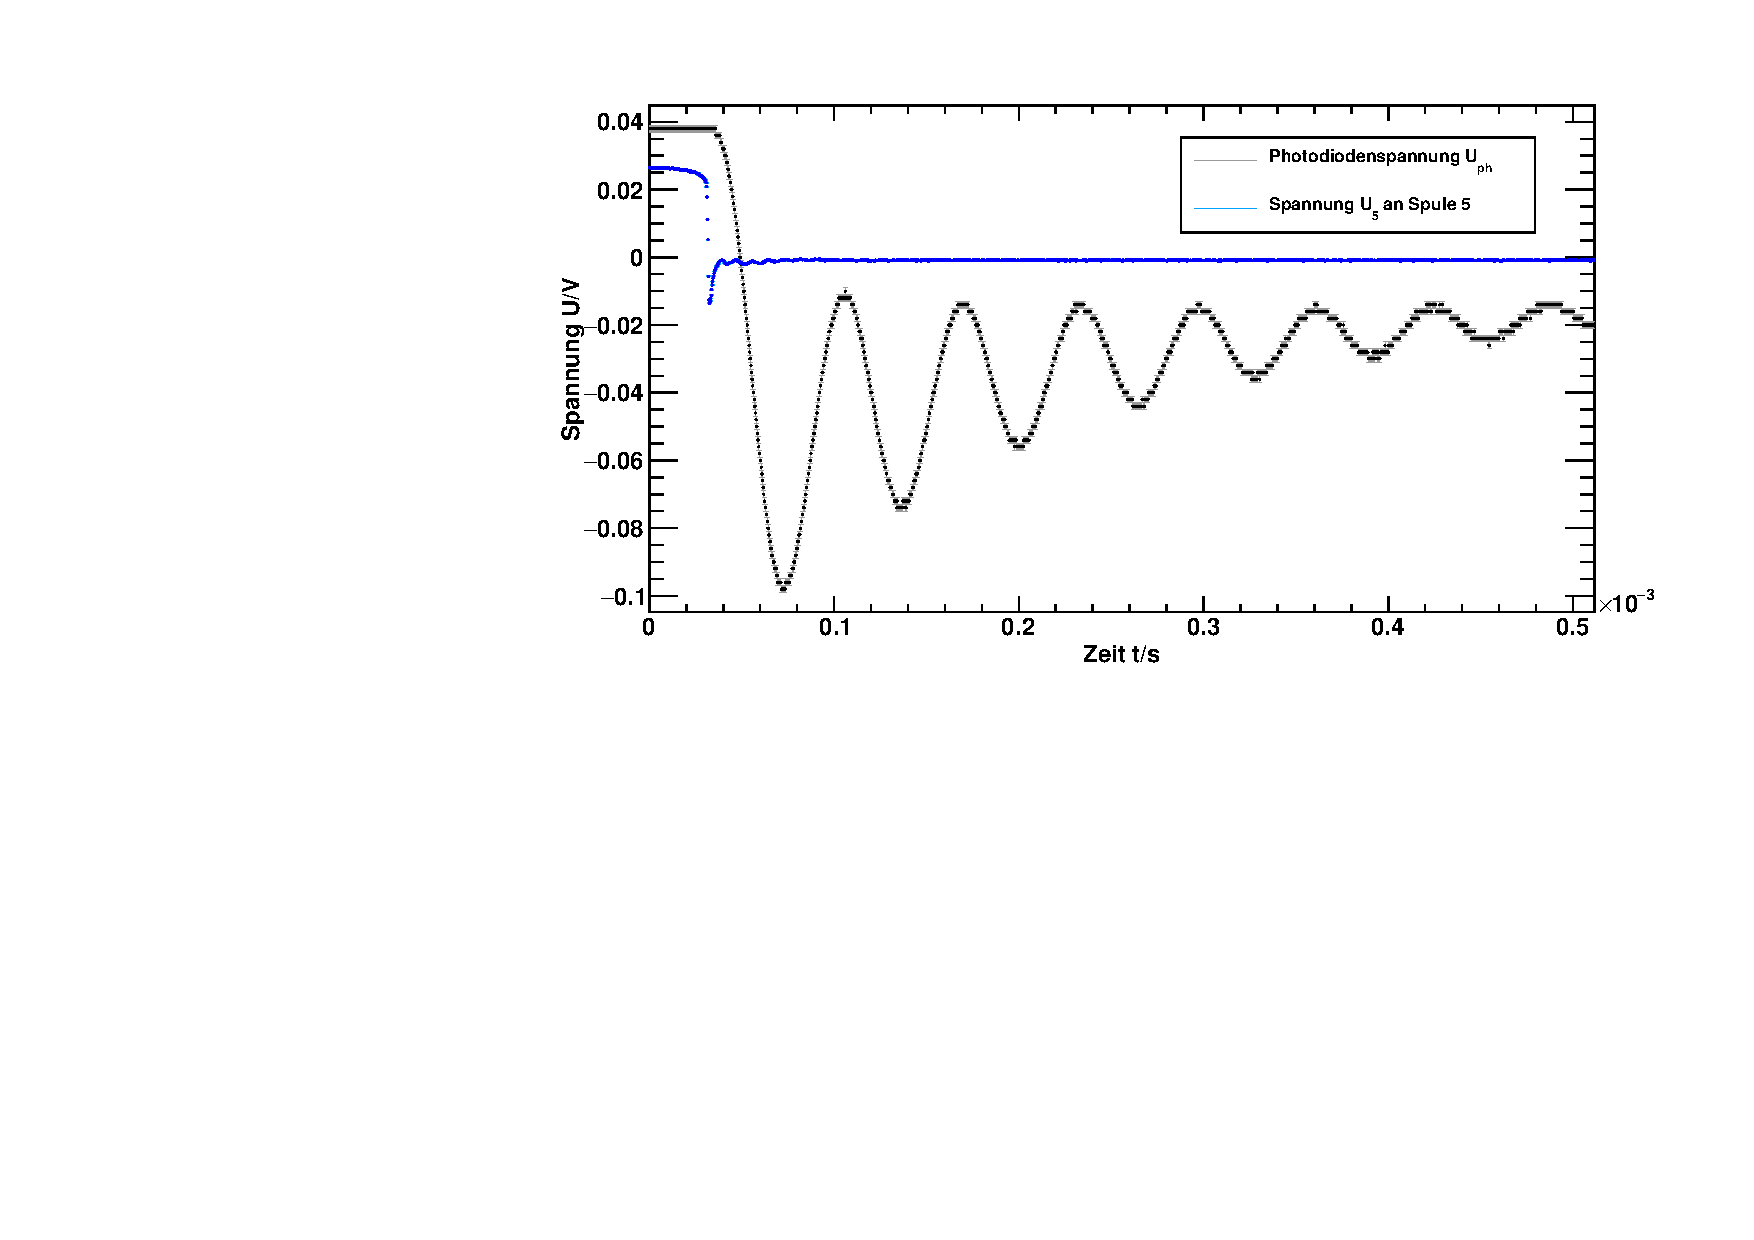
\includegraphics[width=\textwidth]{../img/part4/02-63-7mA-087mA.pdf}
        \caption{Spinpräzession des Rubidiumensembles (\rb{85}), sichtbar in der Transmissionsoszillation der Messzelle.
        Der Strom zur Kompensation des Vertikalfeldes beträgt bei der Messung $I_4$=87\,mA,
        das Erdmagnetfeld ist also fast vollständig kompensiert und die Präzessionsfrequenz dementsprechend gering.}
        \label{img:spp:expl1}
    \end{center}
\end{figure}

\begin{figure}[htb]
    \begin{center}
        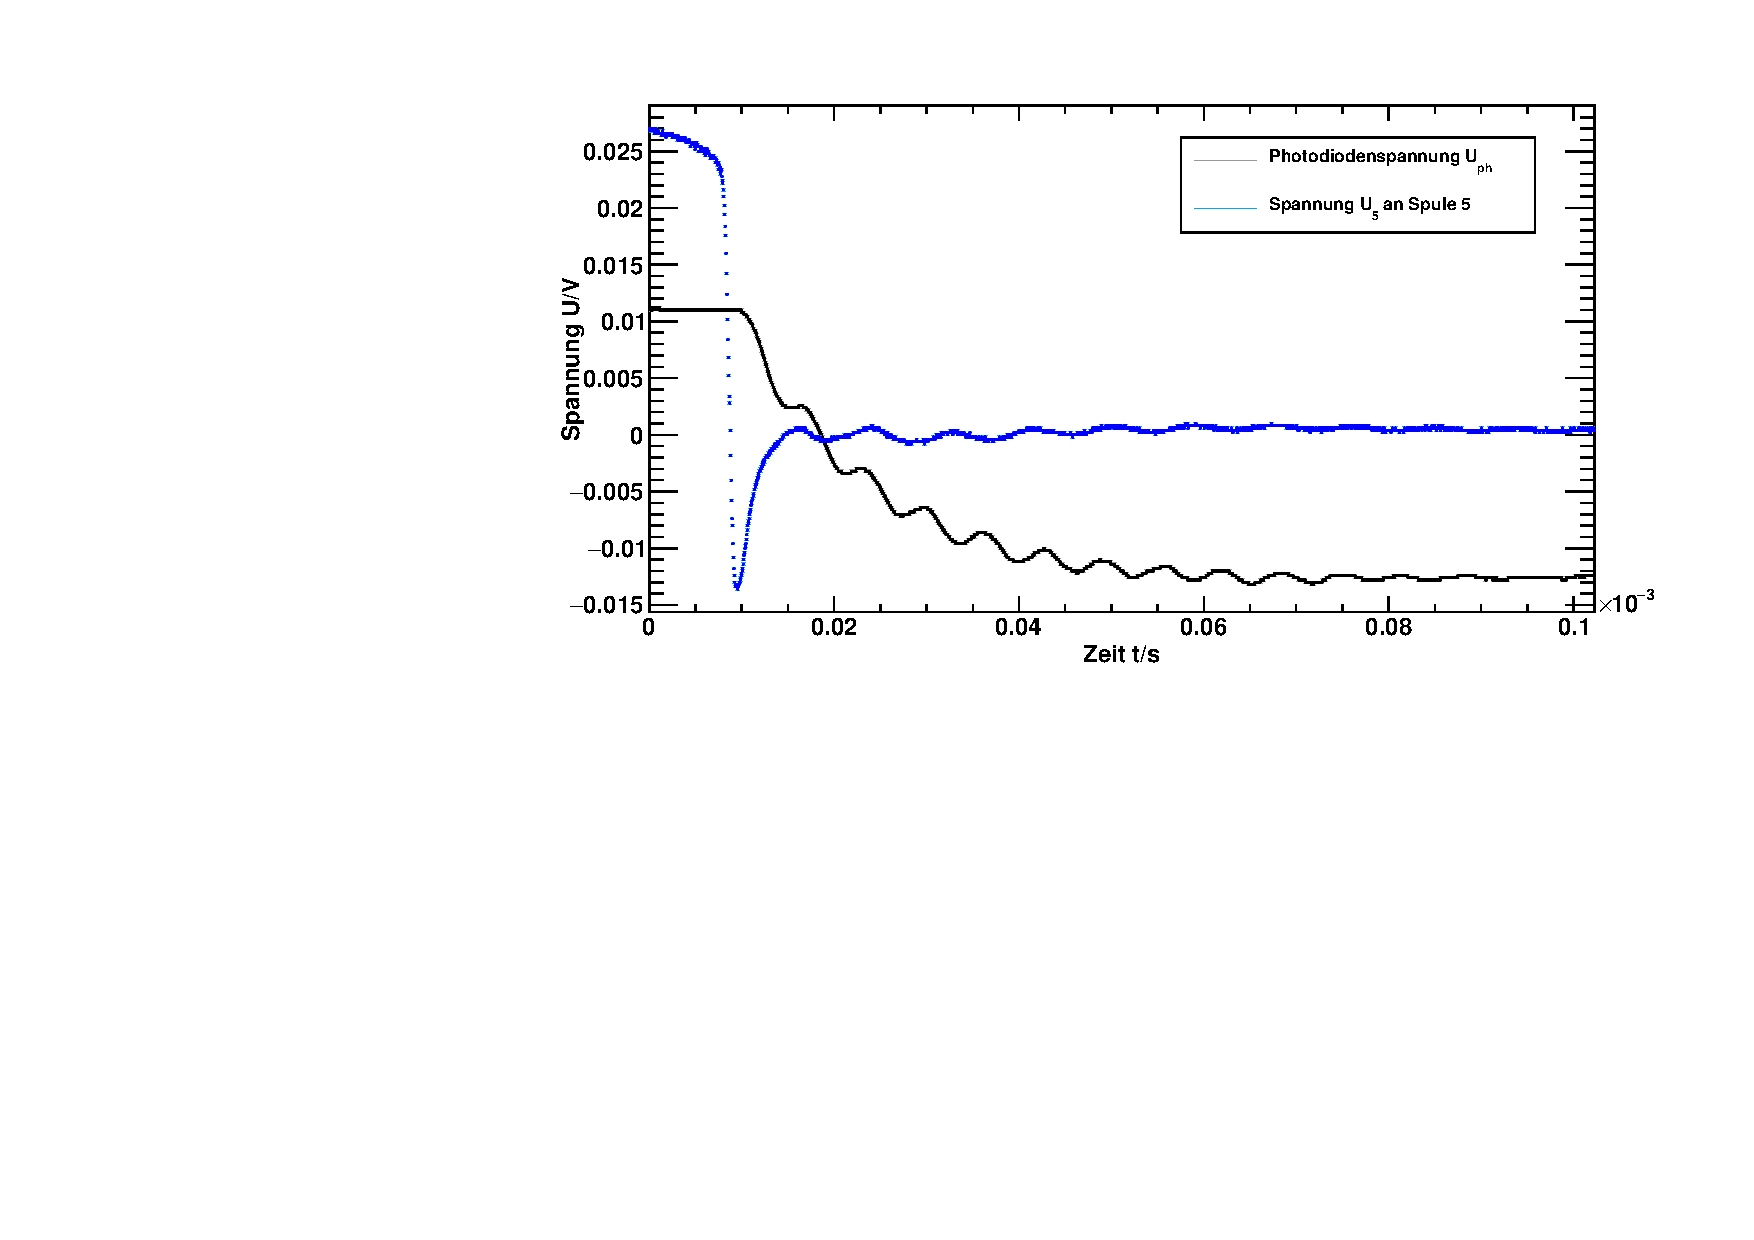
\includegraphics[width=\textwidth]{../img/part4/02-63-7mA-020mA.pdf}
        \caption{Spinpräzession des Rubidiumensembles (\rb{85}) bei $I_4$=20\,mA Kompensationsstrom.
        Das Signal ist höherfrequent als auf \autoref{img:spp:expl1} und besitzt eine kleinere Amplitude.
        Das Auffinden dieses Signals ist daher deutlich schwieriger.}
        \label{img:spp:expl2}
    \end{center}
\end{figure}

\autoref{img:spp:expl1} und \autoref{img:spp:expl2} zeigen zwei der gemessen Spinpräzessionssignale.
Auf der ersten Abbildung ist ein Signal gezeigt, das entsteht, wenn das Erdmagnetfeld fast
vollständig kompensiert ist. Dieses Signal besitzt eine große Amplitude und lässt sich relativ leicht
mit dem Oszilloskop finden.
Wird der Kompensationsstrom $I_4$ nun langsam verringert, lassen sich auch Signale mit höherer Frequenz finden.
Ohne Kompensation des Feldes ist das Präzessionssignal
nur mit einer Mittelwertbildung von 128 oder mehr Messwerten
auf dem Oszilloskop messbar. Für die einzelnen Messungen wird jeweils eine geeignete Mittlung gewählt.

Zur Bestimmung der Präzessionsperiodendauer $T$ bzw. der
Präzessionsfrequenz $f$ werden die Zeitkoordinaten $t_1$ und $t_2$
von zwei möglichst weit voneinander entfernten Maxima per Hand abgelesen und durch
die Zahl $n$ der dazwischenliegenden Perioden geteilt:
\begin{equation}
    T=\frac{t_2-t_1}{n}=f^{-1}, \qquad s_f = n \frac{\sqrt{s_{t_2}^2 + s_{t_1}^2}}{ \left( t_2 -t_1 \right)^2 }
\end{equation}
Der relative Fehler auf die abgelesenen Zeiten wurde auf $\frac{s_{t_i}}{t_i}=0.01$ abgeschätzt,
$n$ ist nicht fehlerbehaftet.

Aus dem Strom durch Spule~4 wird mit \autoref{tab:inductorItoB} das erzeugte vertikale Magnetfeld
$B_\text{S,v}$ berechnet. Der Fehler auf den Strom beträgt $s_{I_4}=1$\,mA.

Die Abhängigkeit der Präzessionsfrequenz $f$ vom Vertikalfeld $B_\text{S,v}$ ist auf
\autoref{img:spp:SPPRb85} gezeigt.
Ein erster Fit erfolgt gemäß \autoref{eq:gr:spinpräz} mit
\begin{equation}
    f_1(B_\text{S,v})=\alpha \cdot |B_\text{E,v}-B_\text{S,v}| \ \, ,
\end{equation}
wobei $B_\text{E,v}$ die Vertikalkomponente des Erdmagnetfelds bezeichnet und
$\alpha$ eine Proportionalitätskonstante.
Es ist deutlich erkennbar, dass das lineare Modell (rot) die Messwerte nur beschreiben kann,
wenn sich die Richtung des effektiven Vertikalfeldes
$B_\text{E,v} \text{\,-\,} B_\text{S,v}$ in der Messreihe nicht umdreht;
die Messpunkte für $B_\text{S,v}$\,>\,40\,\textmu T liegen weit vom Modell entfernt.
Der Wert für das reduzierte \textchi$^2$ beträgt 8.0 und ist damit deutlich zu hoch.

\begin{figure}[H]
    \begin{center}
        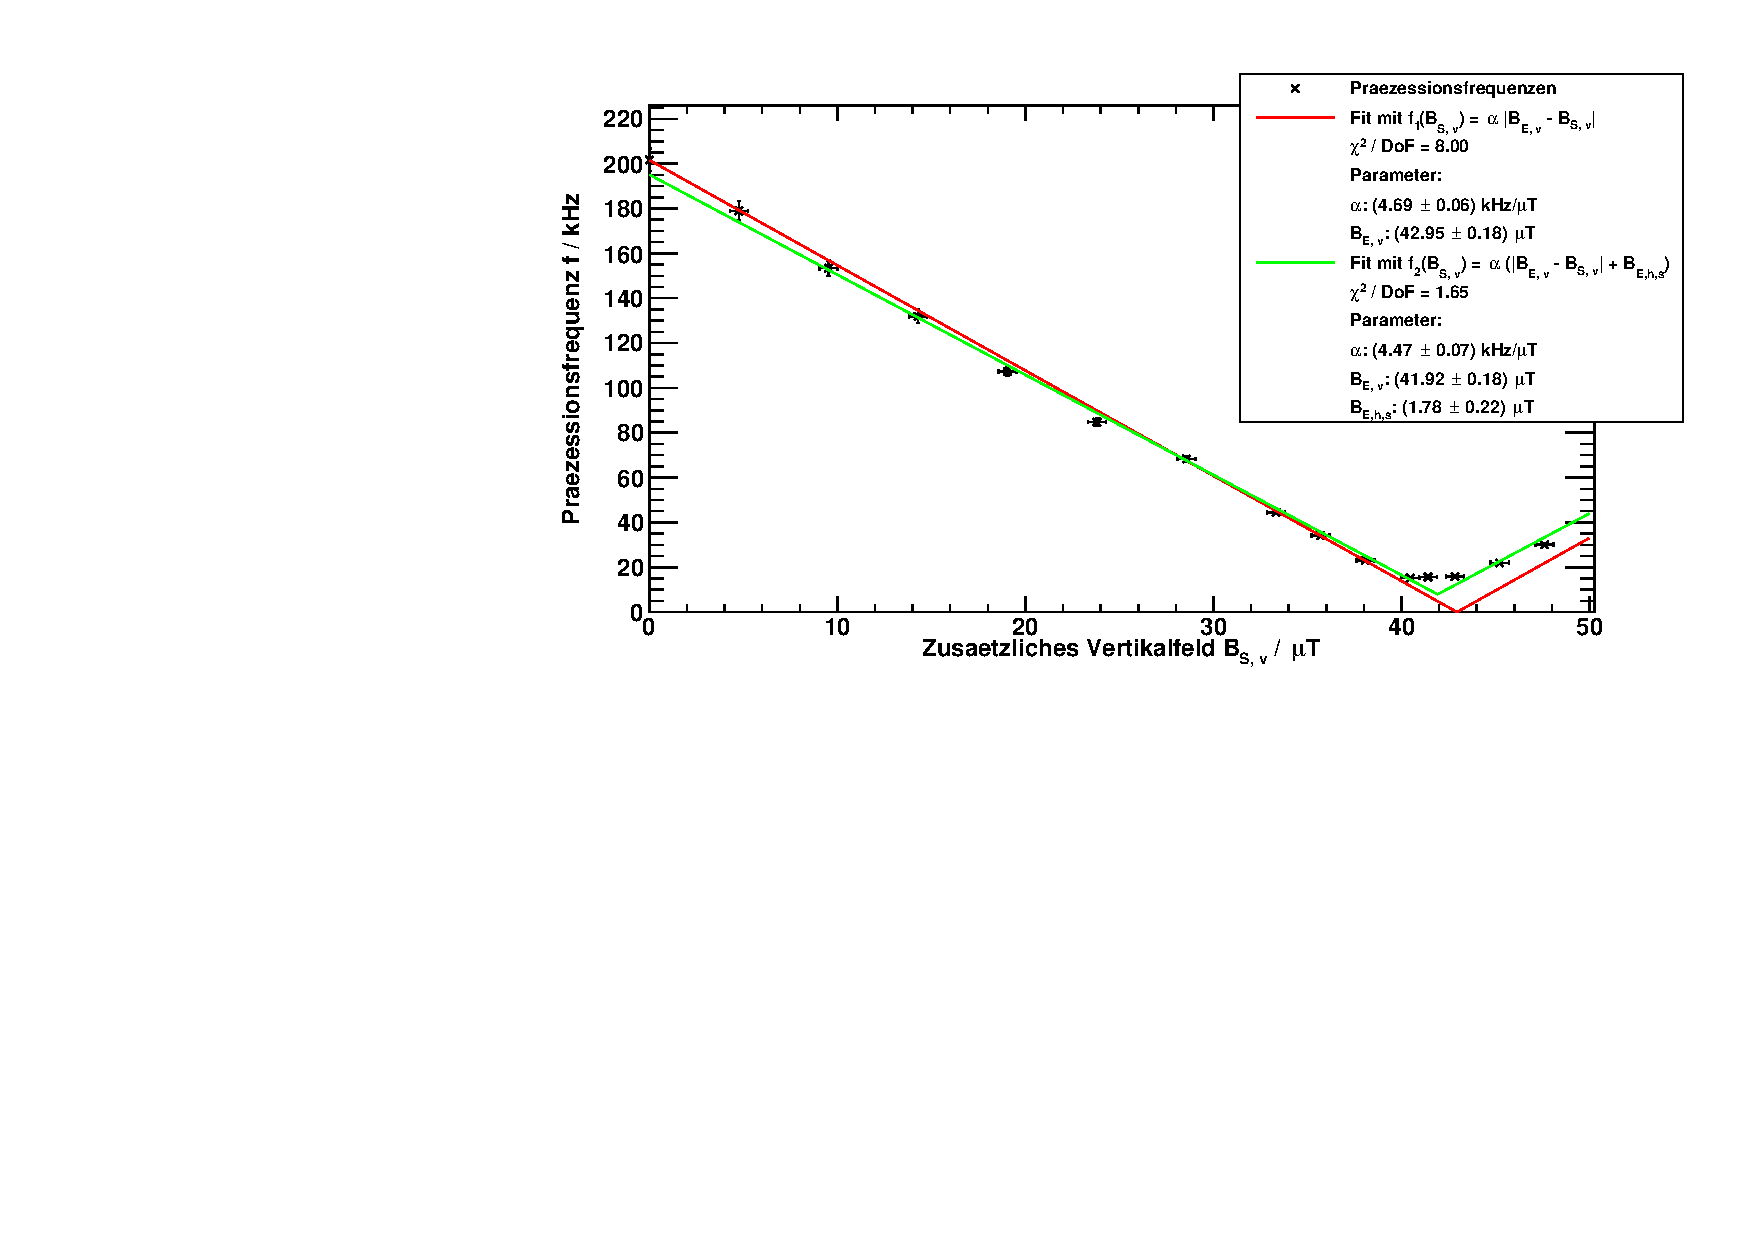
\includegraphics[width=\textwidth]{../img/part4/Rb85.pdf}
        \caption{Spinpräzessionsfrequenz $f$ von \rb{85} in Abhängigkeit
        vom zusätzlichen vertikalen Magnetfeld $B_\text{S,v}$, das dem Erdmagnetfeld überlagert ist.
        Der Fit erfolgt mit einem einfachen Modell sowie unter Berücksichtigung des
        nichtkompensierten Erdmagnetfelds~$B_\text{E,h,s}$.}
        \label{img:spp:SPPRb85}
    \end{center}
\end{figure}

Aus diesem Grund wird ein modifiziertes Modell verwendet, das der Tatsache Rechnung trägt,
dass der Horizontalanteil des Erdmagnetfelds senkrecht zum Strahl $B_\text{E,h,s}$
während der Messung unkompensiert bleibt:
\begin{equation}
    f_2(B_\text{S,v})=\alpha \cdot (|B_\text{E,v}-B_\text{S,v}| + B_\text{E,h,s}) \ \, .
\end{equation}
Dieses Modell eignet sich zur Beschreibung der Messdaten, das reduzierte \textchi$^2$ beträgt 1.7.

Die Auswertung erfolgt analog für das Isotop \rb{87} (\autoref{img:spp:SPPRb87}).
In \autoref{tab:spp:fitres} sind die Ergebnisse aller vier Fits aufgeführt.

\begin{table}[H]
    \caption{Ergebnisse der Fits der Präzessionsfrequenzen
    für die Komponenten des Erdmagnetfeldes und die Proportionalitätskonstante $\alpha$ (theoretische Werte aus \autoref{eq:gr:alpha}).}
    \begin{center}
        \begin{tabular}{|c|c|c|c|c|}
            \hline
            Fit						& $B_\text{E,v}$ / \textmu T	& $B_\text{E,h,s}$ / \textmu T	& $\alpha$ / kHz \textmu T$^{-1}$	& $\alpha^\text{theo}$ / kHz \textmu T$^{-1}$   \\ \hline
   \rb{85}: \emph{Modell 1}	& 42.95$\,\pm\,$0.18			& $-$ 							& 4.69$\,\pm\,$0.06					& 4.665											\\ \hline
\rb{85}: \emph{Modell 2}	& 41.92$\,\pm\,$0.18			& 1.8$\,\pm\,$0.2				& 4.47$\,\pm\,$0.07					& 4.665											\\ \hline
\rb{87}: \emph{Modell 1}	& 41.85$\,\pm\,$0.18			& $-$ 							& 7.33$\,\pm\,$0.10					& 6.998											\\ \hline
\rb{87}: \emph{Modell 2}	& 41.74$\,\pm\,$0.18			& 1.8$\,\pm\,$0.2				& 6.65$\,\pm\,$0.12					& 6.998											\\ \hline

        \end{tabular}
    \end{center}
    \label{tab:spp:fitres}
\end{table}

\begin{figure}[H]
    \begin{center}
        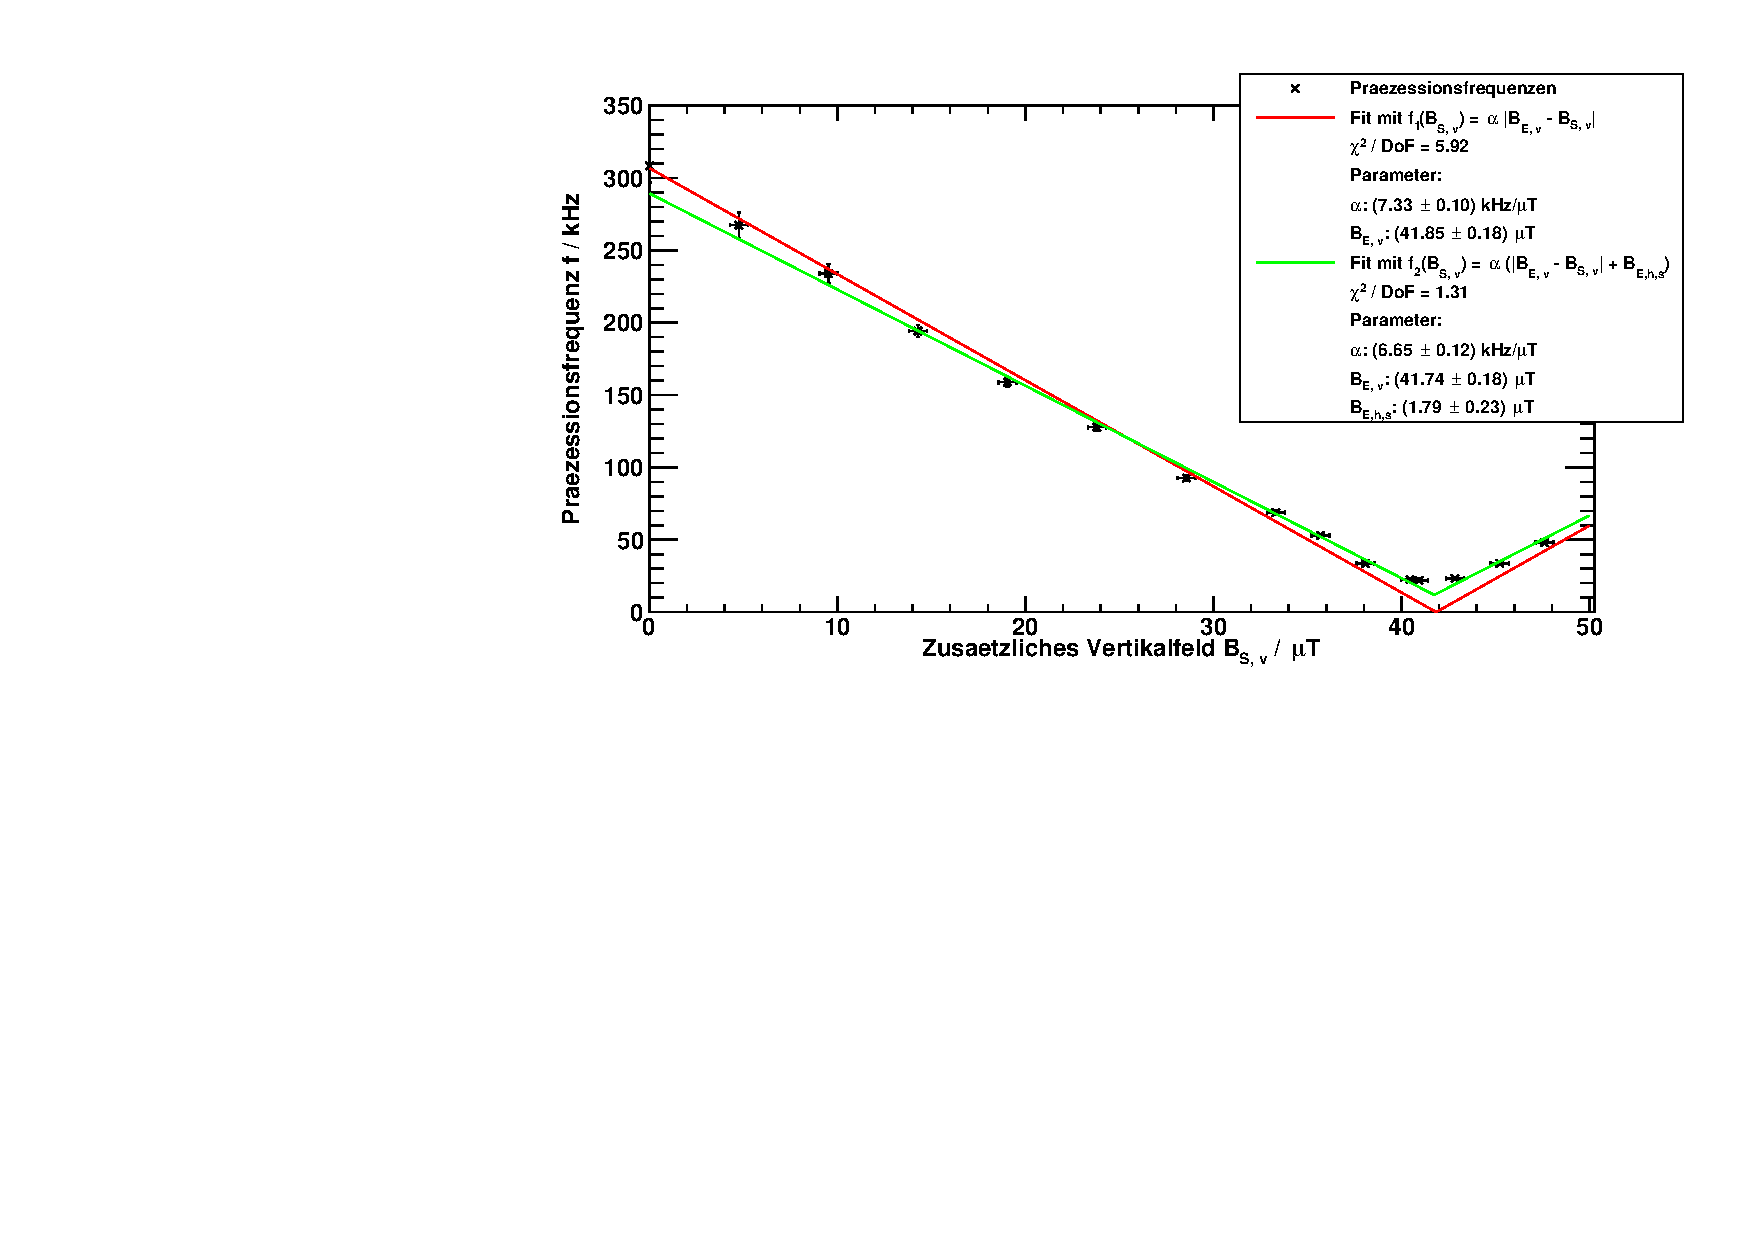
\includegraphics[width=\textwidth]{../img/part4/Rb87.pdf}
        \caption{Spinpräzessionsfrequenz $f$ von \rb{87} in Abhängigkeit
        vom zusätzlichen vertikalen Magnetfeld $B_\text{S,v}$ und Fit mit einfachem und komplexeren Modell.}
        \label{img:spp:SPPRb87}
    \end{center}
\end{figure}

Die Ergebnisse für das vertikale Erdmagnetfeld $B_\text{E,v}$ stimmen nicht mit dem Literaturwert (\autoref{eq:litvalBver}) überein.
Allerdings sind die beiden Werte von Modell~2 konsistent.
Dies spricht dafür,
dass der Literaturwert die Verhältnisse am Aufbau nicht beschreibt.
Die Ursache dafür könnten Magnetfelder von elektrischen Geräten im Gebäude sein,
die dem Erdmagnetfeld überlagert sind.


Die Ergebnisse für die Proportionalitätskonstante $\alpha$ zeigen Abweichungen von bis zu
4\,\textsigma\ vom theoretischen Wert.
Dies könnte zum einen daran liegen, dass der Fehler auf die Messwerte unterschätzt wurde,
zum anderen an einer Ungenauigkeit des Umrechnungsfaktors vom Spulenstrom $I_4$ in das Magnetfeld $B_\text{S,v}$.

Zusätzlich erhält man im zweiten Modell einen Wert für die unkompensierte Horizontalkomponente des Erdmagnetfelds $B_\text{E,h,s}$.
Die Ergebnisse für die beiden Isotope stimmen in Wert und Fehler überein.
Da in \autoref{sect:doppelresauswertung} der Wert für die Horizontalkomponente des Erdmagnetfelds in
Strahlrichtung ($\bar{B}_\text{hor}$ = (12.3$\,\pm\,$0.6)\,\textmu T) bestimmt wurde,
lässt sich nun mit einfachen trigonometrischen Überlegungen der Winkel $\varphi_\text{diff}$ berechnen,
um den der Strahlengang von Norden abweicht:
\begin{equation}
    \varphi_\text{diff} = \arctan\left( \frac{B_\text{E,h,s}}{\bar{B}_\text{hor}} \right)
    = (8.3 \pm 1.0)^\circ  \ \, .
\end{equation}

Der Messaufbau wurde also um 8$^\circ$ gegen den Uhrzeigersinn gedreht
(für die Drehrichtung entschieden wir uns nach einem Blick auf eine Landkarte)
und die Messung an \rb{85} erneut durchgeführt.
\autoref{img:spp:SPPRb87gedr} zeigt die Messung und den Fit mit den beiden Modellen.
Das einfache Modell ist jetzt auch zur Beschreibung der Messdaten geeignet.
Die Parameter von Modell~2 stimmen mit denen von Modell~1 überein;
$B_\text{E,h,s}$ ist innerhalb der Fehlergrenzen 0.

Die Verwendung des erweiterten Modells für die ersten beiden Messungen lieferte also hier eine korrekte Vorhersage
für die Abweichung der Ausrichtung des Strahlengangs von Norden;
die Drehung des Strahlengangs um 8$^\circ$ führte zu einem vollständigen Verschwinden der Horizontalkomponente
des Magnetfelds.

\begin{figure}[H]
    \begin{center}
        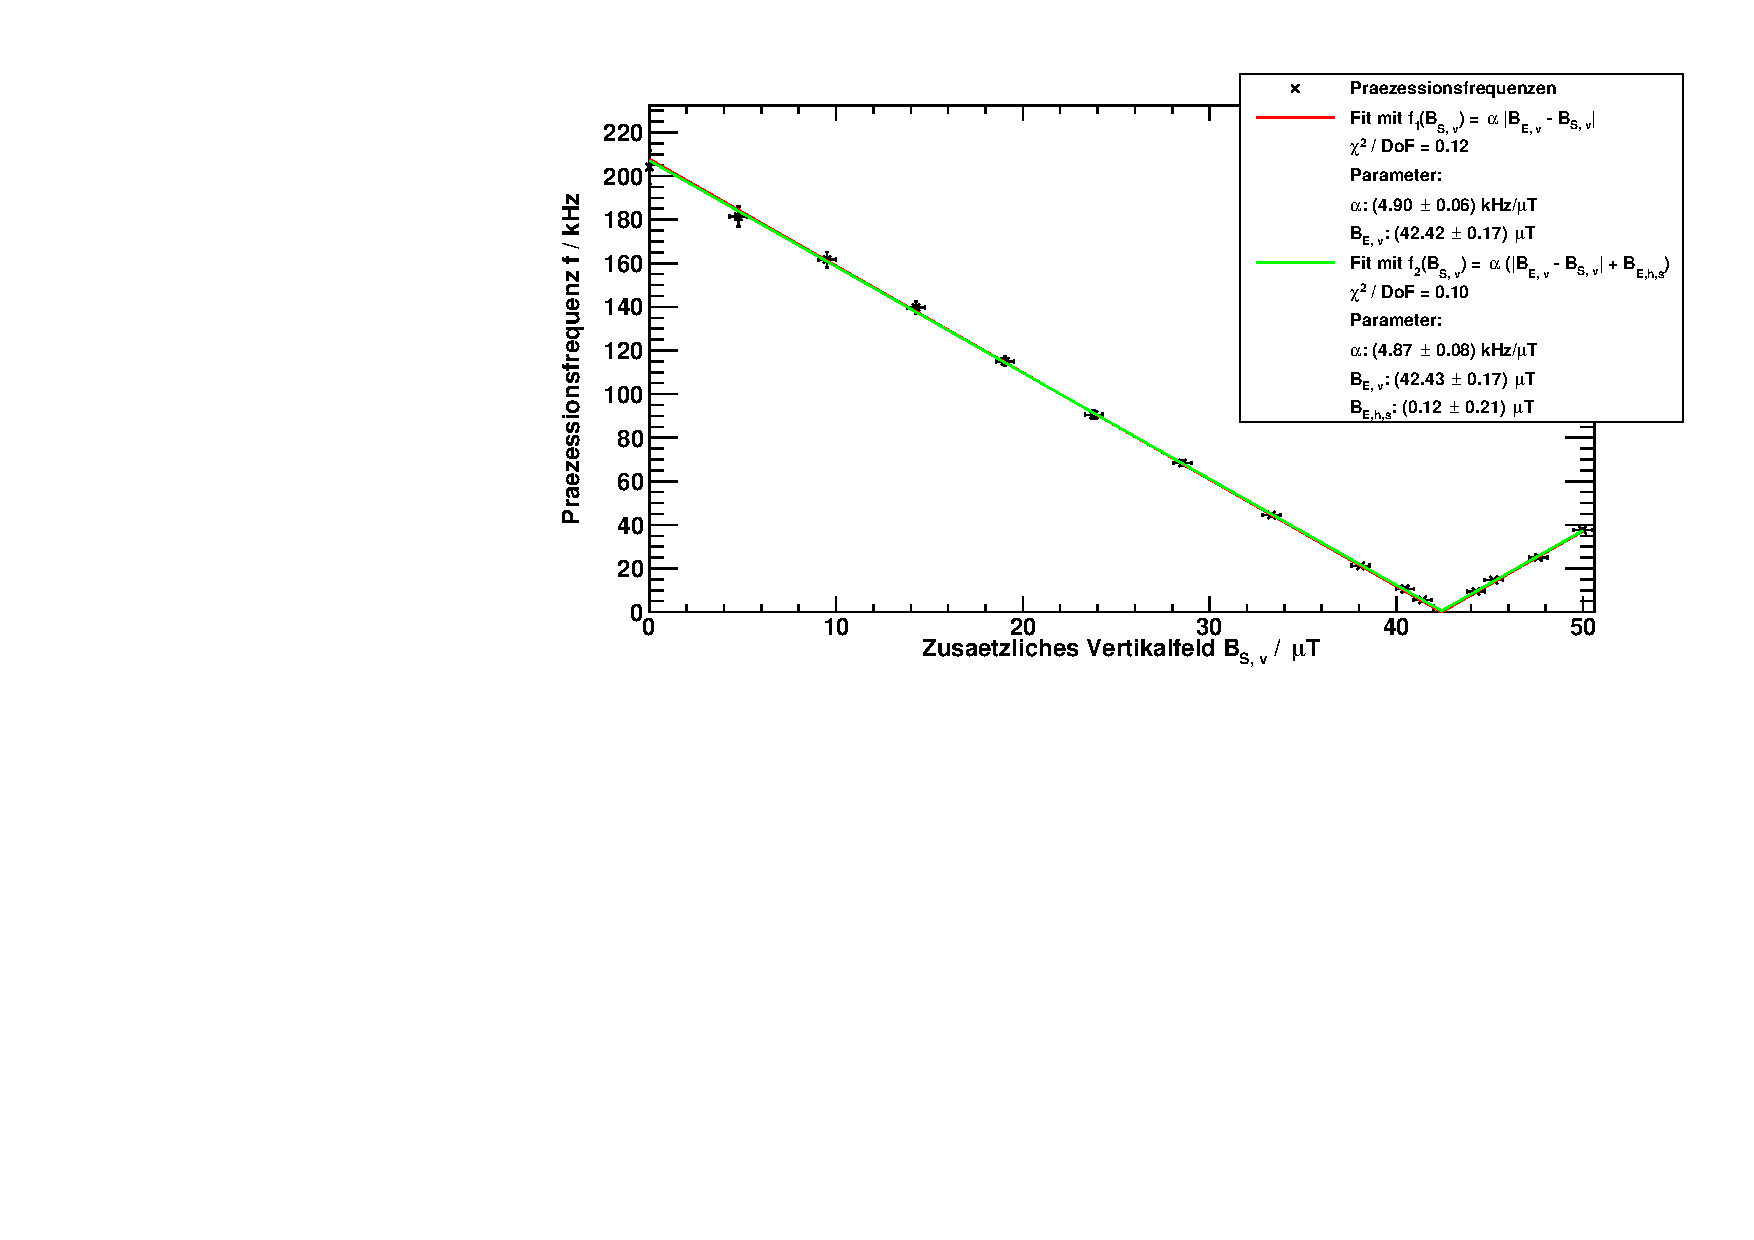
\includegraphics[width=\textwidth]{../img/part4/Rb85_gedreht.pdf}
        \caption{Spinpräzessionsfrequenz $f$ von \rb{85} in Abhängigkeit
        vom zusätzlichen vertikalen Magnetfeld $B_\text{S,v}$
        nach Drehung des Messaufbaus um 8$^\circ$ gegen den Uhrzeigersinn.}
        \label{img:spp:SPPRb87gedr}
    \end{center}
\end{figure}

Als Fitparameter erhält man mit Modell~1
\begin{equation}
    B_\text{E,v} = (42.37\,\pm\,0.14)\,\text{\textmu T} \qquad \text{und} \qquad \alpha = (4.92\,\pm\,0.05)\,\text{kHz } \text{\textmu T}^{-1} \ \, .
\end{equation}
Der Wert für das vertikale Erdmagnetfeld stimmt aus dem oben erwähnten Grund nicht mit dem Literaturwert überein,
ist aber innerhalb von zwei Standardabweichungen konsistent mit den Ergebnissen der ersten beiden Messungen.
Gründe für die starke Abweichung des Parameters $\alpha$ vom theoretischen Wert wurden oben genannt.

Durch Drehung des Aufbaus um Winkel $\varphi$ erfolgt eine weitere Untersuchung der Horizontalkomponente des Erdmagnetfelds 
mit der Überprüfung der Winkelabhängigkeit der Präzessionsfrequenz.
Für sie gilt
\begin{equation}
    f(\varphi) = \alpha \cdot B_\text{E,h,n} \cdot |\sin(\varphi)| =:\beta \cdot |\sin(\varphi)|\ \, ,
\end{equation}
mit der Horizontalkomponente $B_\text{E,h,n}$ des Erdmagnetfelds in Nordrichtung.
\autoref{img:spp:Winkelabhängigkeit} zeigt die Messergebnisse und den Fit mit obiger Gleichung.
Leider erlaubten die Abmessungen des Aufbaus eine Drehung nur im Bereich von -10$^\circ$ bis 10$^\circ$,
so dass für den Sinus auch die Kleinwinkelnäherung verwendet werden könnte.

\begin{figure}[H]
    \begin{center}
        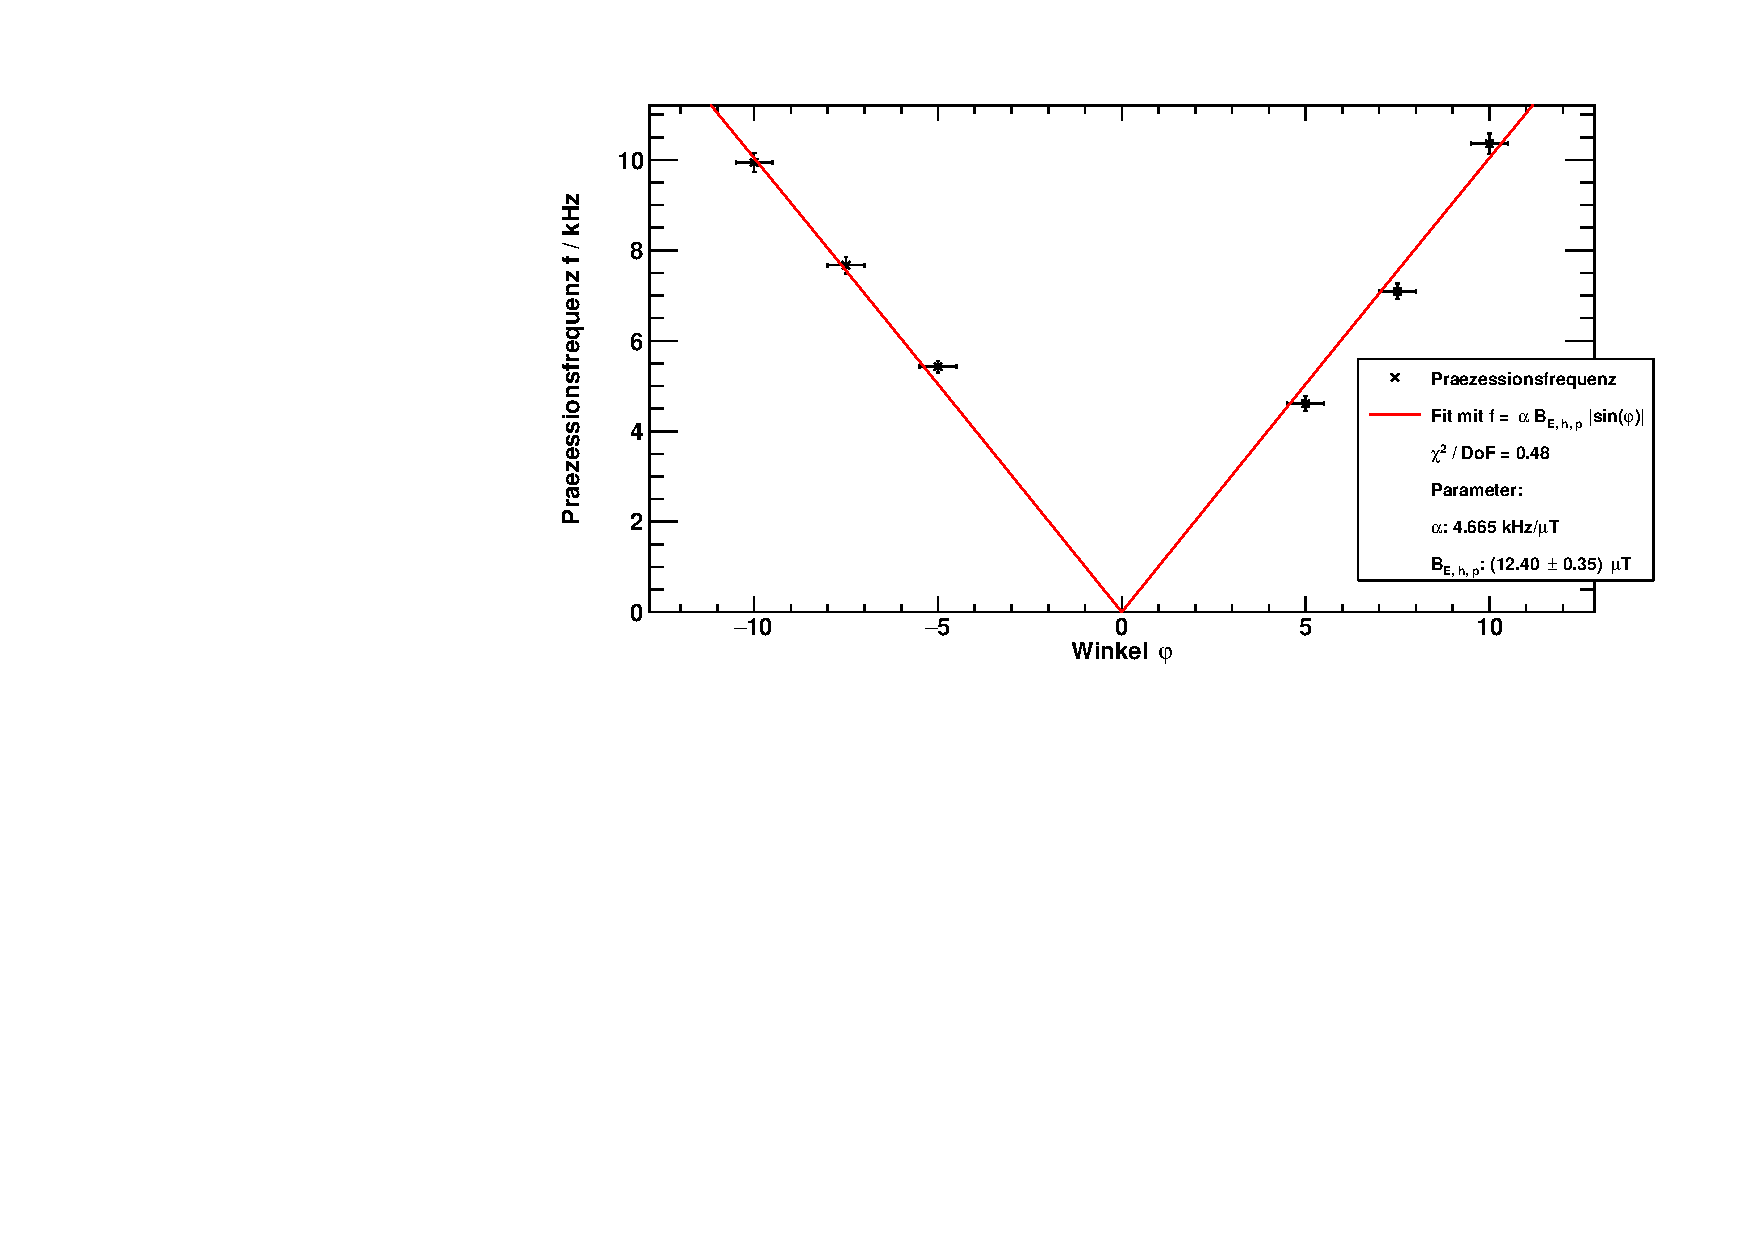
\includegraphics[width=\textwidth]{../img/part4/winkel.pdf}
        \caption{Abhängigkeit der Spinpräzessionsfrequenz $f$ von der Ausrichtung des Messaufbaus im Erdmagnetfeld.}
        \label{img:spp:Winkelabhängigkeit}
    \end{center}
\end{figure}

Im Fit wurde eine eventuelle Abweichung des Nullpunkts der Winkelskala
von der Nordrichtung $\varphi_0$ berücksichtigt;
diese ist im Rahmen der Fehlergrenzen verschwindend.


Die Horizontalkomponente des Erdmagnetfelds in Nordrichtung $B_\text{E,h,n}$ lässt sich
mit trigonometrischen Überlegungen aus der gemessenen Horizontalkomponente in Strahlrichtung $\bar{B}_\text{hor}$
(aus \autoref{sect:doppelresauswertung}) und der Komponente senkrecht zum Strahl $B_\text{E,h,s}$ bestimmen.
Sie beträgt
\begin{equation}
    B_\text{E,h,n} = \sqrt{\bar{B}_\text{hor}^2+B_\text{E,h,s}^2}=(12.4 \pm 0.6)\,\text{\textmu T} \ \, .
\end{equation}

Damit erhält man aus der Steigung der Fitgeraden $a$ für die Proportionalitätskonstante
\begin{equation}
    \alpha = \frac{\beta}{B_\text{E,h,n}} = (4.7\pm0.3)\,\text{kHz } \text{\textmu T}^{-1} \ \, .
\end{equation}

Dieser Wert stimmt im Rahmen seines (großen) Fehlers mit dem theoretischen Wert überein.
Der Fehler auf $\alpha$ könnte verkleinert werden,
wenn die Messung über einen größeren Winkelbereich durchgeführt würde,
so dass die sinusförmige Abhängigkeit deutlich wird.
